\documentclass[11pt]{beamer}
\usetheme[progressbar=frametitle]{metropolis}
\setbeamertemplate{frame numbering}[fraction]
\useoutertheme{metropolis}
\useinnertheme{metropolis}
\usefonttheme{metropolis}
\usecolortheme{spruce}
\setbeamercolor{background canvas}{bg=white}

\definecolor{mygreen}{rgb}{.125,.5,.25}
\usecolortheme[named=mygreen]{structure}

\title{Floating-point}
%\subtitle{subtitle here}
\author{Van Duc NGUYEN}
\institute{\textbf{Viettel IC Design}}
\date{}
\begin{document}
\metroset{block=fill}
\begin{frame}
\titlepage
\end{frame}
\begin{frame}[t]{Over View}
\begin{enumerate}
\item Introduce
\item Floating-point Representation
\item IEEE 754 floating-point standard for binary
\item Floating-point Arithmetic
\item Implementation in FPGA
\end{enumerate}
\end{frame}
\begin{frame}[t]{1.Introduce}
Why Floating-point?
\begin{enumerate}
\item Advantages
\begin{itemize}
\item Dynamic range\\
with fixed-point $DR_{fxpt}=r^n-1$.\\
with floating-point $DR_{flpt}=\frac{M_{max}*b^{E_max}}{M_{min}*b^{E_min}}$
\end{itemize}
\item Disadvantages
\begin{itemize}
\item Precision
\item Roundoff error
\item Complex implementation
\end{itemize}
\end{enumerate}
\end{frame}
\begin{frame}[t]{2.Floating-point Representation}
Form represent a floating-point number:\\
\begin{center}
    \begin{figure}[htp]
    \begin{center}
     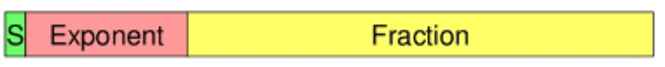
\includegraphics[scale=.5]{image/fig21}
    \end{center}
    \label{reffig21}
    \end{figure}
\end{center}
With three fields:
\begin{itemize}
\item Sign bit:S (0 is positive and 1 is negative)
\item Fraction:F (Significand or mantissa)
\item Exponent:E
\end{itemize}
Value of floating-point number:{$(-1)^S*{F}*B^{\pm{E}}$}\\
with B
\footnote{The base B is implicit.(base is 2,10..)}
\end{frame}
\begin{frame}{Normalized and Denormalized representation}
\begin{itemize}
\item Normalized:$\pm{1.mmm...m}*B^{\pm{E}}$\\
\item Denormalized:$\pm{0.mmm...m}*B^{E_{min}}$
\end{itemize}
\begin{center}
    \begin{figure}[htp]
    \begin{center}
     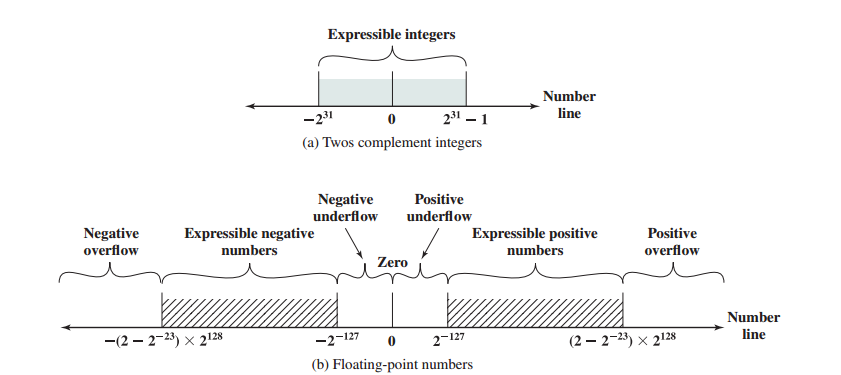
\includegraphics[scale=.5]{image/fig2}
    \end{center}
    %\caption{Cái sẽ hiển thị bên dưới hình}
    \label{reffig2}
    \end{figure}
\end{center}
\end{frame}
\begin{frame}[t]{3.IEEE 754 Floating-point Standard for binary}
The three basic format have bit lengts of 32,64 and 128 bits:
\begin{center}
    \begin{figure}[htp]
    \begin{center}
     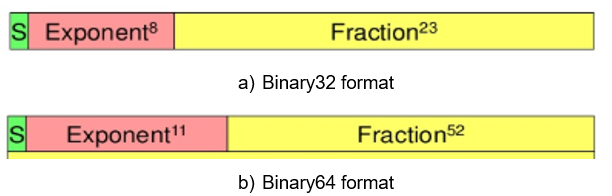
\includegraphics[scale=.5]{image/fig20}
    \end{center}
    %\caption{Binary32 format}
    \label{reffig20}
    \end{figure}
\end{center}

For a normalized floating-point number:
\begin{center}
    \begin{figure}[htp]
    \begin{center}
     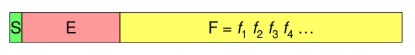
\includegraphics[scale=.7]{image/fig24}
    \end{center}
    %\caption{Cái sẽ hiển thị bên dưới hình}
    \label{reffig24}
    \end{figure}
\end{center}
Value of floating-point:$\pm{1.f_1f_2f_3f_4...f_l}*2^{\pm{E}}$\\
\end{frame}
\begin{frame}[t]{IEEE 754 Format Paremeter}
\begin{center}
    \begin{figure}[htp]
    \begin{center}
     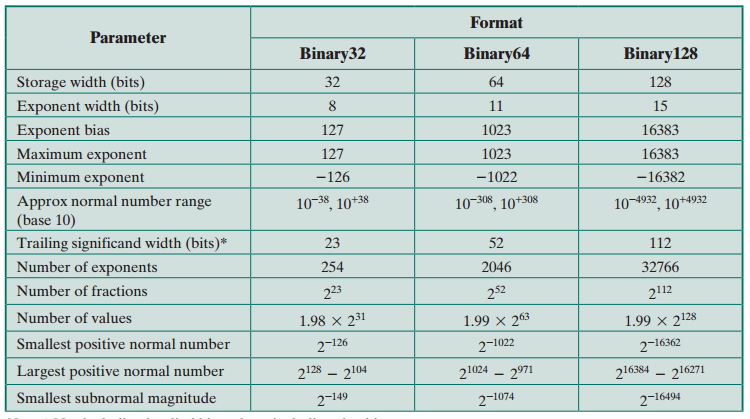
\includegraphics[scale=.5]{image/fig4}
    \end{center}
    %\caption{Cái sẽ hiển thị bên dưới hình}
    \label{reffig4}
    \end{figure}
\end{center}
\end{frame}
\begin{frame}[t]{Biased Exponent Representation}
IEEE 754 use biased representation for the exponent:
\begin{itemize}
\item Value of exponet= val(E)=E - Bias(Bias is a constant)
\item Bias is computed base on $bias=2^{k-1}-1$ (with k is lengths of bit)
\item For signle precision,k=8 and bias=127,value of E(biased)=val(E)+127.
\end{itemize}
\end{frame}
\begin{frame}[t]{Special value}
IEEE 754 define some special value as NaN,Infinity to represent for underflow,overflow and not a number...\begin{center}
    \begin{figure}[htp]
    \begin{center}
     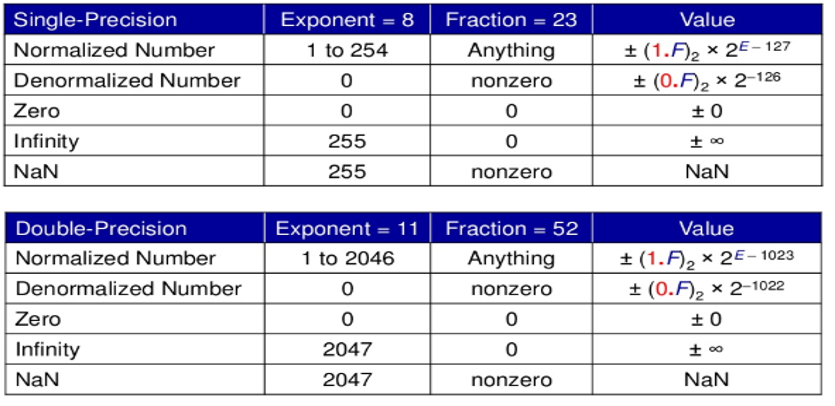
\includegraphics[scale=.5]{image/fig25}
    \end{center}
   %\caption{Cái sẽ hiển thị bên dưới hình}
    \label{reffig25}
    \end{figure}
\end{center}

\end{frame}
\begin{frame}[t]{3.Floating-point Arithmetic}
Basic opreations for floating-point arithmetic:
\begin{center}
    \begin{figure}[htp]
    \begin{center}
     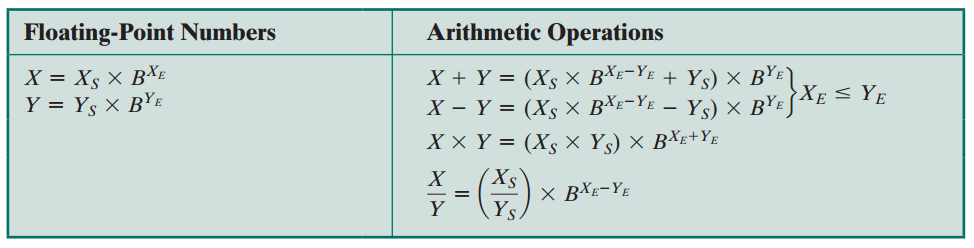
\includegraphics[scale=.4]{image/fig26}
    \end{center}
    %\caption{Cái sẽ hiển thị bên dưới hình}
    \label{reffig26}
    \end{figure}
\end{center}
\end{frame}
\begin{frame}[t]{Addition and Subtration}
    \begin{figure}[htp]
    \begin{center}
     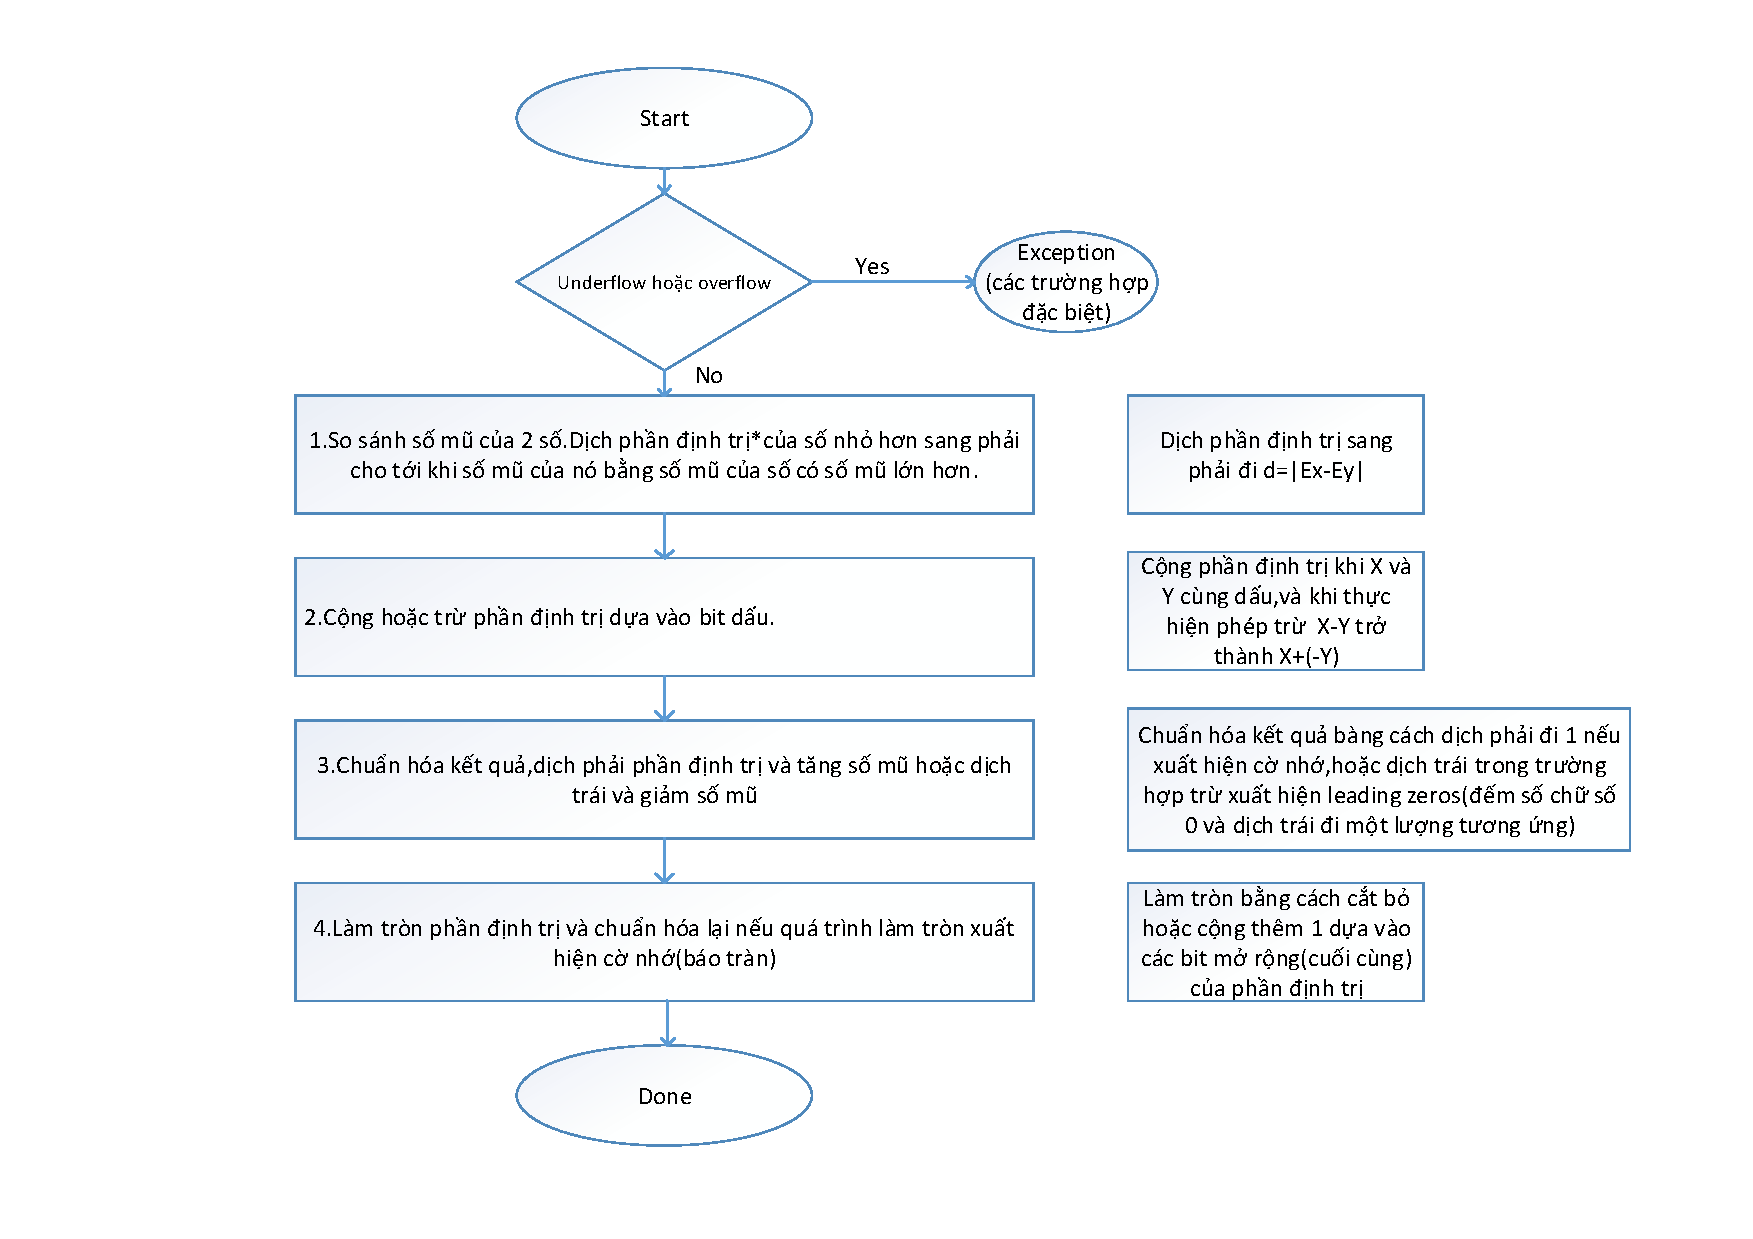
\includegraphics[scale=.37]{image/pesucodeadd}
    \end{center}
    %\caption{Cái sẽ hiển thị bên dưới hình}
    \label{refpesucodeadd}
    \end{figure}
\end{frame}
\begin{frame}[t]{4.Implementation in FPGA}

\end{frame}
\begin{frame}[t]{5.Conclusion}

\end{frame}
\end{document}
